\documentclass{article}
\usepackage[utf8]{inputenc}
\usepackage{amsmath,amssymb}
\usepackage{makecell}
\usepackage[a4paper, total={6in, 9in}]{geometry}
\usepackage{authblk}
\usepackage{graphicx}
\graphicspath{{.}}
\author{Zihan Zhao}
\affil{1001103708}
\title{Homework 1}
\date{}
\begin{document}
\maketitle
\section{}
\renewcommand{\thesubsection}{(\alph{subsection})}
\subsection{}
First determine $E[Z]$
\begin{align*}
  E[Z] &= E[(X-Y)^2]\\
  &= E[(X^2 - 2XY + Y^2]\\
  &= E[X^2] - E[2XY] + E[Y^2]\\
  &= E[X^2]  2E[X]E[Y] + E[Y^2]\\
\end{align*}
Since X and Y both are variables from uniform distribution in $[0,1]$, $E[x] = E[Y]$ and $E[X^2] = E[Y^2]$. Therefore,
\begin{align*}
    continue:\\
    E[Z] &= 2E[X^2] + 2E[X]^2\\
    &= 2\int^1_0 x^2f(x)dx - 2(\int^1_0 xf(x)dx)^2
\end{align*}
Note that $f(x)$ is the pdf of X. So $f(x) = \frac{1}{1-0} = 1$. Therefore,
\begin{align*}
    continue:\\
    E[Z] &= 2\int^1_0 x^2dx - 2(\int^1_0 xdx)^2\\
    &= 2*\frac{1}{3} - 2*(\frac{1}{2})^2\\
    &= \frac{1}{6} = 0.16667
\end{align*}
Second determine $Var[Z]$
\begin{align*}
    Var[Z] &= E[Z^2]-E[Z]^2\\
    &= E[(X-Y)^4]-(\frac{1}{6})^2\\
    &= E[X^4-4X^3Y+6X^2Y^2-4XY^3+Y^4]-(\frac{1}{6})^2\\
    &= E[X^4]-4E[X^3]E[Y]+6E[X^2]E[Y^2]-4E[X]E[Y^3]+E[Y^4]-(\frac{1}{6})^2\\
\end{align*}
Since X and Y both are variables from uniform distribution in $[0,1]$, $E[x] = E[Y]$, $E[X^2] = E[Y^2]$, $E[X^3] = E[Y^3]$, and $E[X^4] = E[Y^4]$ Therefore,
\begin{align*}
    Var[Z] &= 2E[X^4]-8E[X^3]E[X]+6E[X^2]^2-(\frac{1}{6})^2\\
    &= 2\int^1_0 x^4f(x)dx - 8(\int^1_0 x^3f(x)dx)(\int^1_0 xf(x)dx) + 6(\int^1_0 x^2f(x)dx)^2-(\frac{1}{6})^2\\
    &= 2*\frac{1}{5} - 8*\frac{1}{4}*\frac{1}{2} + 6(\frac{1}{3})^2-(\frac{1}{6})^2=\frac{7}{180}=0.38889
\end{align*}
\subsection{}
First determine $E[R]$. Since $X_1,..,Y_d$ are i.i.d, $(X_1-Y_1)^2,...,(X_d-Y_d)^2$ are independent. Therefore,
\begin{align*}
    E[R] &= E[\sum_{i = 1}^{d}Z_i]\\
    &= \sum_{i = 1}^{d}E[Z_i]\\
    &= dE[Z] = \frac{d}{6}
\end{align*}
Second determine $Var[R]$. Since $Z_1,..,Z_d$ are independent, $Cov(Z_i,Z_j)=0$ where i and j are arbitrary picks from 1 to d. Therefore,
\begin{align*}
    Var[R] &= Var[\sum_{i = 1}^{d}Z_i]\\
    &= \sum_{i = 1}^{d}Var[Z_i] + 2\sum_{i<j}^{d}Cov[Z_i,Z_j]\\
    &= dVar[Z] = \frac{7d}{180}
\end{align*}
\section{}
\subsection{}
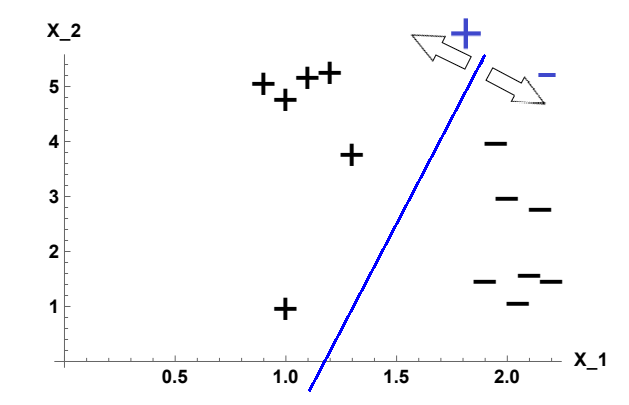
\includegraphics{2a.png}
\subsection{}
No, it is not unique.
\subsection{}
0. The left side of the boundary marks "+" and the right side marks "-". All "+" points are in left side and all "-" points are in right side.
\subsection{}
\label{sec:2d}
As $\lambda$ approaches $\infty$, $J(w)$ heavily depends on $\lambda\omega_0^2$. In order to minimize $\lambda\omega_0^2$, $\omega_0$ should be 0. So the boundary should pass through (0,0). The sketch is shown below.\\
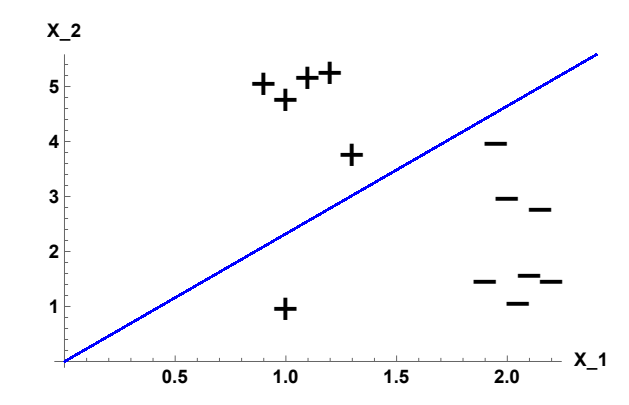
\includegraphics{2d.png}
\subsection{}
1. The upper side of the boundary marks "+" and the down side marks "-". All "+" points are in left side except one point is at down side. All "-" points are in right side. So the error is 1.
\subsection{}
Similar with \ref{sec:2d}, in order to minimize $\lambda\omega_1^2$, $\omega_1$ should be 0. So the boundary line is $\omega_0 + \omega_2x_2 = 0$. It should be a horizontal line. The sketch is shown below.\\
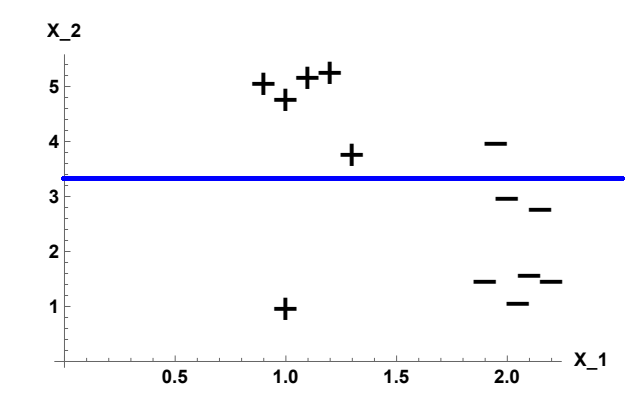
\includegraphics{2f.png}
\subsection{}
2. The upper side of the boundary marks "+" and the down side marks "-". All "+" points are in left side except one point is at down side. All "-" points are in right side except one point is at upper side. So the error is 2.
\subsection{}
Similar with \ref{sec:2d}, in order to minimize $\lambda\omega_2^2$, $\omega_2$ should be 0. So the boundary line is $\omega_0 + \omega_1x_1 = 0$. It should be a vertical line. The sketch is shown below.\\
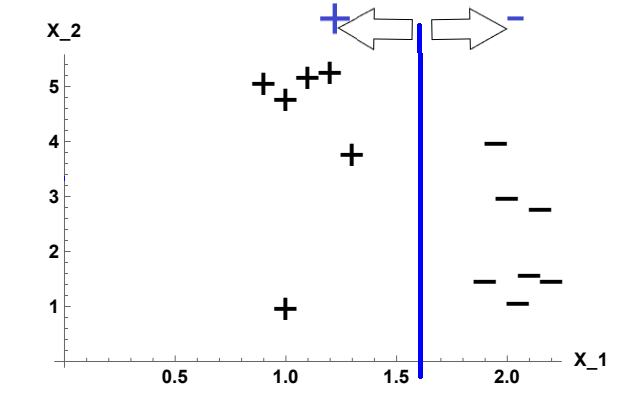
\includegraphics{2h.png}
\subsection{}
0. The left side of the boundary marks "+" and the right side marks "-". All "+" points are in left side and all "-" points are in right side.
\section{}
\subsection{}
Since $p(x)$ is possibility mass, $0\leq p(x)\leq 1$. Therefore,
\begin{align*}
    p(x)&\leq 1\\
    \frac{1}{p(x)} &\leq 1\\
    \log (\frac{1}{p(x)}) &\geq 1 \geq 0\\
\end{align*}
since $p(x) \geq 0$,
\begin{align*}
    p(x)\log (\frac{1}{p(x)}) &\geq 0\\
    H(X) = \sum_{x}^{} p(x) \log (\frac{1}{p(x)}) &\geq 0
\end{align*}
\subsection{}
In order to prove $KL(p||q)\geq 0$, it is equivalent to prove $\sum_{x}^{X}p(x)\log (\frac{p(x)}{q(x)})\geq 0$. Let's define new variable Y which is $y=f(x)=\frac{q(x)}{p(x)}$. Then let's define a new function $\phi(y)=-\log y$, which is convex function. According to Jensen's Inequality,
\begin{align*}
    E[\phi(Y)] &\geq \phi(E[Y])\\
    \sum_{x}^{X}p(x)\phi(f(x)) &\geq \phi(E[Y])\\
    -\sum_{x}^{X}p(x)\log(\frac{q(x)}{p(x)}) &\geq \phi(E[Y])\\
    \sum_{x}^{X}p(x)\log(\frac{p(x)}{q(x)}) &\geq \phi(E[Y])\\
    KL(p||q) &\geq \phi(E[Y])\\
    KL(p||q) &\geq \phi(E_x[f(x)])\\
    KL(p||q) &\geq \phi(\sum_{x}^{X}p(x)\frac{q(x)}{p(x)})\\
    KL(p||q) &\geq \phi(\sum_{x}^{X}q(x))\\
    KL(p||q) &\geq \phi(1)\\
    KL(p||q) &\geq -\log(1)\\
    KL(p||q) &\geq 0
\end{align*}
\subsection{}
In order to show that
\begin{align*}
    I[Y;X] = KL(p(x,y)||p(x)p(y))
\end{align*}
On left side,
\begin{align*}
    I[Y;X] &= H(Y) - H(Y|X)\\
    &= \sum_{y}p(y)\log(\frac{1}{p(y)}) - (-\sum_{y}\sum_{x}p(x,y)\log(p(y|x)))\\
    &= \sum_{y}p(y)\log(\frac{1}{p(y)}) + \sum_{y}\sum_{x}p(x,y)\log(p(y|x))
\end{align*}
On right side,
\begin{align*}
    KL(p(x,y)||p(x)p(y)) &= \sum_{y}\sum_{x} p(x,y)\log(\frac{p(x,y)}{p(x)p(y)})
\end{align*}
note that $p(y|x) =\frac{p(x,y)}{p(x)}$
\begin{align*}
    KL(p(x,y)||p(x)p(y)) &= \sum_{y}\sum_{x} p(x,y)\log(\frac{p(y|x)}{p(y)})\\
    &= \sum_{y}\sum_{x} (p(x,y)(\log(p(y|x))+\log(\frac{1}{p(y)})))\\
    &= \sum_{y}\sum_{x} (p(x,y)(\log(p(y|x)))+\sum_{y}\sum_{x}(p(x,y)\log(\frac{1}{p(y)})))\\
    &= \sum_{y}\sum_{x} (p(x,y)(\log(p(y|x)))+\sum_{y}(p(y)\log(\frac{1}{p(y)})))\\
    &= I[Y;X]
\end{align*}
Therefore right side is equal to left side.\\
Done.
\end{document}